\section{Design of Recluse}
\label{sec:protocol} 
The overview of login flow is shown in Figure~\ref{fig:overview}, which contains RP identifier negotiation, dynamic registration and token obtaining. 
\begin{figure}
  \centering
  \includegraphics[width=\linewidth]{fig/Overview.pdf}
  \caption{Overview of System}
  \label{fig:overview}
\end{figure}
The of each phase in login flow is shown as follows:
\begin{itemize}
\item[1.] RP identifier Negotiation: For each SSO procedure, user is going to start negotiation with user. RP identifier is a random number which does not represent any RP, generated by rp-id-generating algorithm. However, the identifier is bound with specific authentication which is able to be confirmed by user and RP.
\item[2.] Dynamic Registration: To make the RP identifier generated by negotiation is valid in IdP, user is to register this identifier with IdP through the dynamic registration API provided by IdP. IdP is going to check whether the identifier is unique and require RP to restart identifier negotiation if the identifier has be used by another RP.
\item[3.] Token Obtaining: After dynamic registration, RP builds the authentication request and redirects it to IdP through user agent. After receiving the request, IdP firstly authenticates user and then issues identity proof for RP, which contains the user id generated through the user-id-generating algorithm. Then IdP redirects the identity to RP through user agent, and RP identify the user through identity proof. 
\end{itemize}

Besides, the prior registration between RP and IdP is required for IdP to verify the basic attributes of RP, such as name, endpoints for identity proof, so that Idp is able to provide the RP certification to RP which includes the unique identifier for each RP and its attributes. With the RP certification, user agent has the ability to verify the RP's endpoint for identity proof and notify user with RP's identity. Additionally, the parameters, prime $P$ (used for user id generating) with its generator $g$, public key of IdP \verb+pk+ is provided in registration as well. Same as RP, user need to register with IdP and IdP generates unique user id for each user. The process of registration is shown as Figure~\ref{fig:registration}
\begin{figure}
  \centering
  \includegraphics[width=\linewidth]{fig/registration.pdf}
  \caption{Prior Registration}
  \label{fig:registration}
\end{figure}



\subsection{Rp-id-generating and User-id-generating algorithm}
The rp-id-generating and user-id-generating algorithm are created based on Discrete Logarithm problem\cite{shiu2007cryptography:}.
IdP carefully chooses a big prime $P$\footnotetext[1]{$P$ is generated as $P=p\cdot q\cdot 2+1$, while $p$ and $q$ are primes.} and its primitive root \verb+g+ as generator for system. When the RP registers with IdP, IdP provides a unique primitive root as the RP's root identifier (called \verb+basic_rp_id+). 

The define of computation is shown as Figure~\ref{fig:define}, based on which the generation of \verb+rp_id+ and \verb+user_id+ is shown as Figure~\ref{fig:generating}, as well as the trapdoor for RP to derive \verb+user_rp_id+ is as shown.
\begin{figure}
  \centering
  \includegraphics[width=\linewidth]{fig/computationdefine.pdf}
  \caption{Define of Computation}
  \label{fig:define}
\end{figure}

\begin{figure*}
  \centering
  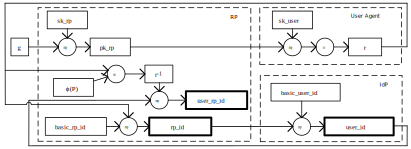
\includegraphics[width=0.8\linewidth]{fig/generating2.pdf}
  \caption{Generation of rp\_id and user\_id}
  \label{fig:generating}
\end{figure*}

For each login process, the user and RP negotiate the temporary RP identifier bound with specific authentication.
While starting a login procedure, there is Diffie-Hellman key Exchange\cite{DiffieH76} between RP and user, through which the random $r$ is generated. However, to make sure that there is $r^{-1}$, that $r\cdot r^{-1}=1 mod \phi(P)$, $r$ should be the relative prime of $\phi(P)$, so that if $r$ is even $r$ should be added by one. Although there is little possibility that $r$ is the multiple of $p$ or $q$, it is not considered in the illustration. However, the re-negotiation is required in the practical system if $r$ is the multiple of $p$ or $q$. The RP identifier is generated as: 
$$rp\_id=basic\_rp\_id^r mod P$$
such that $rp_id$ is another primitive element module \emph{p}. And $r^{-1}$ is generated through Extended Euclidean algorithm.

IdP labels each user at IdP with the unique identifier called $baisc\_user\_id$. To generate the specific user identifier for each $rp\_id$, the algorithm is 
$$user\_id=rp\_id^{id} mod P$$
so
$$user\_id=basic\_rp\_id^{r\cdot id}modP$$
While receiving $user\_id$ from IdP, RP can derive the constant user identifier from if
$$user\_rp\_id=user\_id^{r^{-1}} mod P$$
so
$$user\_rp\_id=basic\_rp\_id^{(1 mod \phi(P))\cdot id} mod P$$
so
$$user\_rp\_id=basic\_rp\_id^{id} mod P$$
For single user in a RP, $user\_rp\_id$ is unchanged. However, $user\_rp\_id$s are distinct in each RP because $basic\_rp\_id$s are different in each RP.



\subsection{Login Flow}
User firstly logs in an RP. If RP find that user is unauthenticated, RP is going to negotiate a new client\_id with user. Then user starts dynamic registration and forward the registration result from IdP to RP. If registration succeeds RP will construct a token request and redirect user to IdP. IdP authenticates user and generates an id\_token of user for RP. Id\_token is sent to RP and RP gets user\_rp\_id from id\_token. RP is going to identify the user through user\_rp\_id. The login flow is shown as Figure~\ref{fig:process}
\begin{figure*}
  \centering
  \includegraphics[width=\linewidth]{fig/process.pdf}
  \caption{Login Flow}
  \label{fig:process}
\end{figure*}

%抵抗phishing攻击:一定需要正确的RP参与,攻击者作为中间人
%1.使用IdP提供应用basic_rp_id与url的绑定,user agent保存映射
%缺点:占用空间,user agent需要缓存整个映射
%2.RP与用户通过加密的通道传输redirect_uri

%如果由RP选择basic_rp_id,那么多个rp之间的basic_rp_id有幂次关系,那么就可以关联用户

\subsubsection{Client\_id Negotiation}
An attacker is able to be the man in the middle between RP and user in client\_id negotiation using phishing attack. When a user logs in attacker's website, attacker logs in another RP as a user. In client\_id negotiation, attacker just transmits user and RP's requests and responses to each other. As a result, attacker shares the same client\_id with user and RP and gets a id\_token valid in RP from user.
So besides of generating client\_id, RP has to send its rp\_certificate to user in this phase. It protects user from sending id\_token to malicious opponent. As rp\_certificate contains RP's name, it allows user can identify the real RP's identity when doing login.
\subsubsection{Dynamic Registration}
User generates IdP's registration URL by \emph{iss} from rp\_certificate. 
The client\_id negotiation is described in user-id-generating algorithm. Dynamic registration starts after client\_id negotiation. User generates a random redirect\_uri and sends it to IdP as well as client\_id. IdP checks the uniqueness of client\_id and sends the result success or fail back. If registration fails, user is going to restart client\_id negotiation. Otherwise user will forward the registration response to RP.  
\subsubsection{Obtaining Token}
Token Obtaining: After dynamic registration, RP builds the authentication request and redirects it to IdP through user agent. User agent verifies the validation of the endpoint for identity proof and replaces it with the fake one. After receiving the request, IdP firstly authenticates user and then issues identity proof for RP. Identity proof contains the user id which is generated by IdP through the user-id-generating algorithm. Then IdP redirects the identity to the fake endpoint through user agent, who is to intercept the transmission and transmit it to the endpoint claimed in authentication request. 
Id token contains RP's client\_id and user id. Client\_id is provided by RP and user id is generated through sser-id-generating algorithm by IdP. RP is able to get the constant user identity from user id.



RP firstly redirects user to IdP with its token request. User generates IdP's authenticate URL by \emph{iss} from rp\_certificate and compared it with RP's redirect location. If they point the same address, user is going to continue the login.
To keep the advanced protocol same as OpenID Connect 1.0, after authenticating a user IdP is going to redirect the user to the redirect\_uri of RP with id\_token as parameter. As redirect\_uri is random, user stops the redirection. User then sends id\_token to the URL received from client\_token negotiation to defend man-in-the-middle attack. RP gets user\_id from id\_token and gets user\_rp\_id computed from user\_id. If it's the first time user logs in RP, RP is going to finish the registration. Otherwise RP searches user profile through user\_rp\_id. 
%\subsection{Roles' Ability Demands}
%\emph{Demands on IdP}. 